\section{Experiments}


\paragraph{Experimental setup} In all the experiments, we use a U-Net-based architecture with timestep embeddings as proposed in~\citet{ho2020denoising,nichol2021improved}. We train all the models with a linear $\beta$ scheduler and uniform steps sampler to simplify the comparison. All implementation details and hyperparameters are included in the Appendix~\ref{appx:hyperparams} and code repository~\footnote{\url{https://github.com/KamilDeja/analysing_ddgm}}. 
For \ours{}, we use the same architecture for both the diffusion part and the denoising autoencoder. 
We run experiments on three standard benchmarks with different complexity: FashionMNIST~\cite{xiao2017fashion} of gray-scale $28 \times 28$ images, CIFAR-10~\cite{Krizhevsky09learningmultiple} of $32 \times 32$ natural images, and CelebA~\cite{liu2015faceattributes} of $64 \times 64$ photographs of faces. We do not use any augmentations during training for any dataset. We report results for both variational lower bound loss (VLB)~\cite{sohl2015deep} and simplified objective~\cite{ho2020denoising}.
Following~\citet{nichol2021improved} we evaluate the quality of generations with Fréchet Inception Distance (FID)~\cite{heusel2017gans} and distributions Precision (Prec) and Recall (Rec) metrics~\cite{sajjadi2018assessing} that disentangle FID score into two aspects: the quality of generated results (Precision) and their diversity (Recall).

\subsection{Is there a transition in functionality of the backward diffusion process that switches from generating to denoising?}
\label{sect:reasonable_to_use_denoiser}


In Section \ref{sec:analysis}, we investigate how the signal-to-noise ratio and the reconstruction error of a DDGM change with the increasing number of diffusion steps (see Figure \ref{fig:mae_cifar_celeba}). Based on this analysis, we postulate that DDGMs can be divided into two parts: a \emph{denoiser} and a \emph{generator}. To determine the switching point, we propose an experiment that answers the following question: \\
%\begin{wrapfigure}{r}{0.46\textwidth}
%\vskip  -12pt
%    \begin{adjustbox}{center}
%    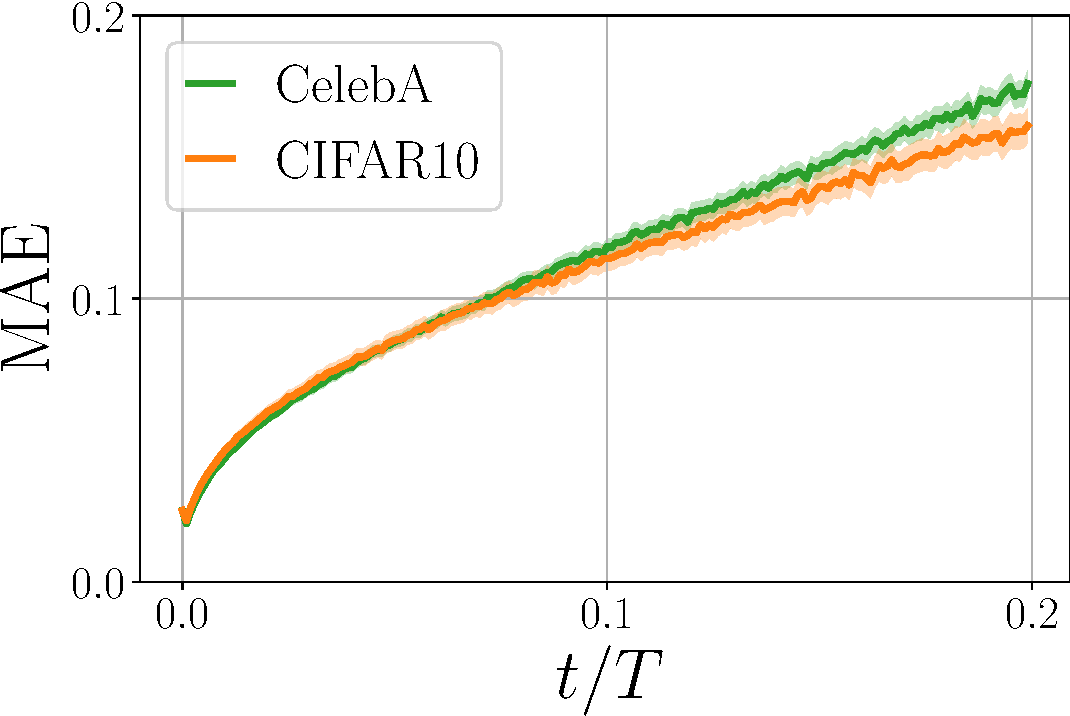
\includegraphics[width=0.4\textwidth]{pics/4_daed/experiments/MAE_step_cifar_celeba.pdf}
%    \end{adjustbox}
%    \vskip -6pt
%    \caption{The MAE for a DDGM trained on CIFAR10 and evaluated on CIFAR10 \& CelebA, with a 0.95 confidence interval.}
%    \label{fig:mae_cifar_celeba}
%    \vskip  -20pt
%    % \end{figure}
%\end{wrapfigure}
\textit{Is there a denoising part of a DDGM that is agnostic to the signal from the data?}
\begin{marginfigure}
	\vspace*{2\baselineskip}
	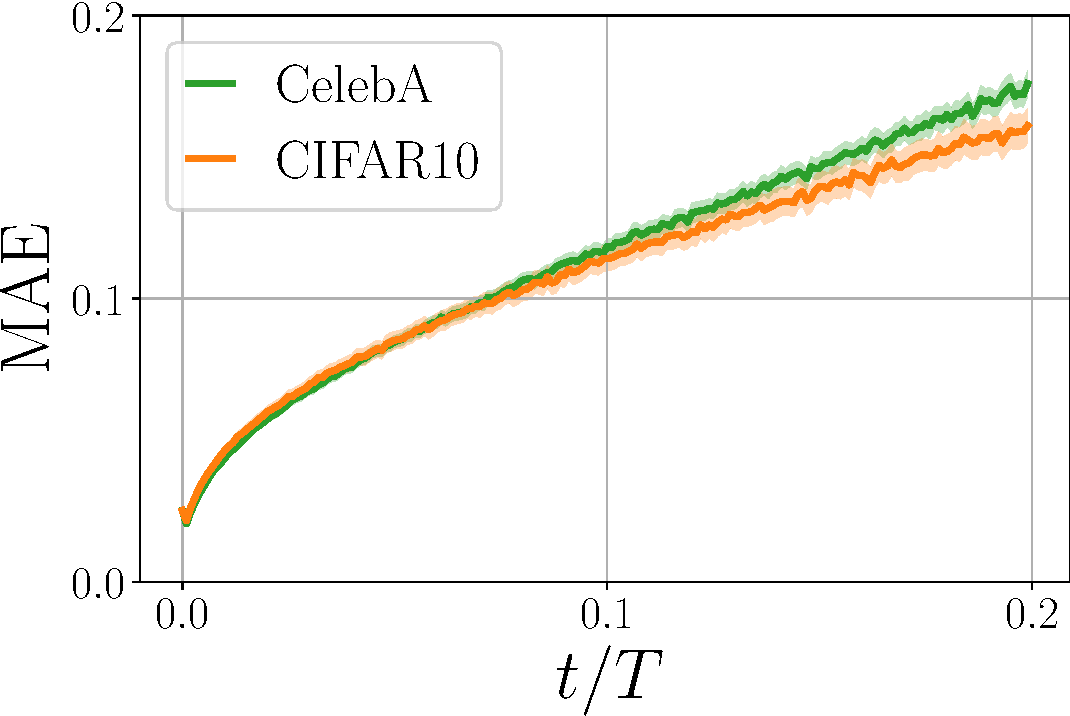
\includegraphics[width=\linewidth]{pics/4_daed/experiments/MAE_step_cifar_celeba.pdf}
	\caption{The MAE for a DDGM trained on CIFAR10 and evaluated on CIFAR10 \& CelebA, with a 0.95 confidence interval.}
	\label{fig:mae_cifar_celeba}
\end{marginfigure}
To that end, we refer once more to the analysis of the reconstruction error (e.g., MAE) from different diffusion steps. This time, however, we compare the quality of reconstructions with a single DDGM model trained on the CIFAR10 dataset and then evaluated on CIFAR10 and CelebA. The result of this experiment is presented in Figure \ref{fig:mae_cifar_celeba}. Interestingly, we notice that for approximately $10\%$ of the initial steps of the DDGM, there is a negligible difference in the reconstruction error between these two datasets. This fact may suggest that, indeed, the model does not require any information about the background data signal in the first steps, and it is capable of denoising corrupted images. However, after this point (about $10\%$ of steps), the reconstruction error starts growing faster for the dataset the model was not trained on. This indicates that information about the domain becomes important and affects performance.


\subsection{How does splitting DDGMs into generative and denoising parts affect the performance?}

The results so far confirm our claims that DDGMs could be divided into denoising and generative parts. Independently of a dataset, there appears to be a transition point at which a DDGM stops generating a corrupted image from noise and starts denoising it in a generative manner. Here, we aim to verify whether it is possible to do a clear split into a denoising part and a generating part. For this purpose, we use the introduced \ours{} approach that consists of a DAE part (the denoiser) and a DDGM (the generator) parameterized by two distinct U-Nets. 

\begin{figure}[t]
    % \vskip -4pt
	\centering
	\begin{tabular}{ccc}
	    	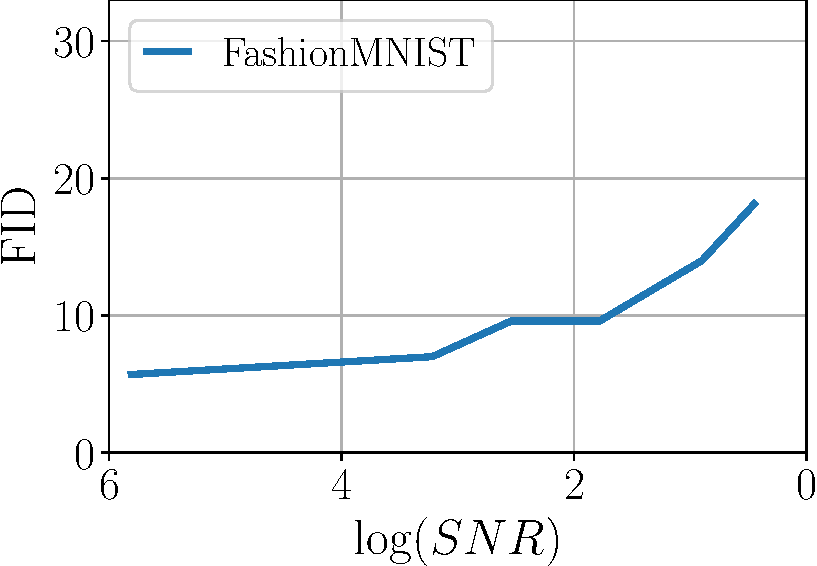
\includegraphics[width=0.3\linewidth]{pics/4_daed/experiments/fid_snr_fmnist.pdf} & %\label{fig:fid_snr_fmnist} &
	     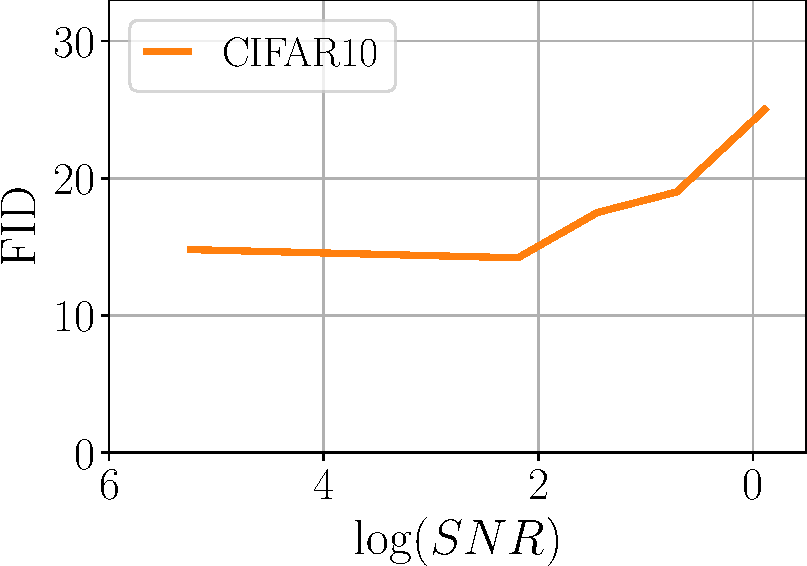
\includegraphics[width=0.3\linewidth]{pics/4_daed/experiments/fid_snr_cifar.pdf} & %\label{fig:fid_snr_cifar10}&
	      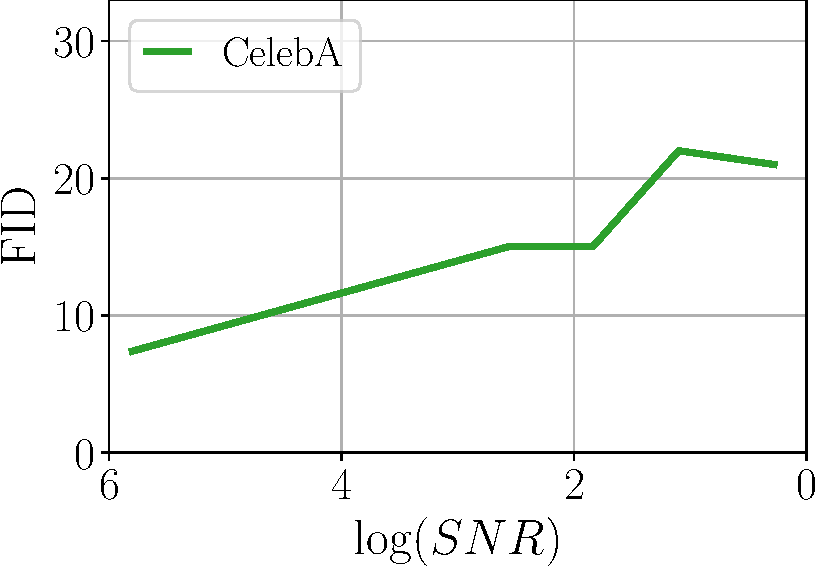
\includegraphics[width=0.3\linewidth]{pics/4_daed/experiments/fid_snr_celeba.pdf} \\ %\label{fig:fid_snr_celeba}\\
	    (a) FashionMNIST& (b) CIFAR10 & (c) CelebA 
	\end{tabular}
% 	\vskip -4pt
	\caption{ The performance (FID) of \ours{} with different switching points with respect to the logarithm of the signal to noise ratio (\protect\ref{eq:snr}) on three different datasets.}
	\label{fig:snr_fid}
	\vskip  -5pt
\end{figure}


First, we consider a situation in which we train a DDGM using the simplified objective (Eq.~\ref{eq:l_t_simple}) and then replace the first steps with a DAE. In other words, we train a \ours{} in two steps: first the DDGM and then the DAE. This experiment aims to check how the decoupling of the DDGM into two parts influences the model performance. In Figure~\ref{fig:snr_fid} we present the dependency between the log-SNR at the splitting point and the FID score. In all cases, the performance of \ours{} is comparable to the DDGM if we replace the DAE with up to the $10\%$ of the steps that correspond to $log(SNR)$ is equal to around $4$. For more complicated datasets like CIFAR10 and CelebA, fewer steps could be replaced. This effect could be explained by the fact that images in these datasets have three channels (RGB), and removing noise is more problematic. That outcome reconfirms our presumptions that it is reasonable to split the DDGM since the final performance is not significantly affected by the division for an adequately chosen splitting point.

% \begin{wrapfigure}{r}{0.6\textwidth}
% \vskip  -10pt
\begin{figure}
    \begin{adjustbox}{center}
    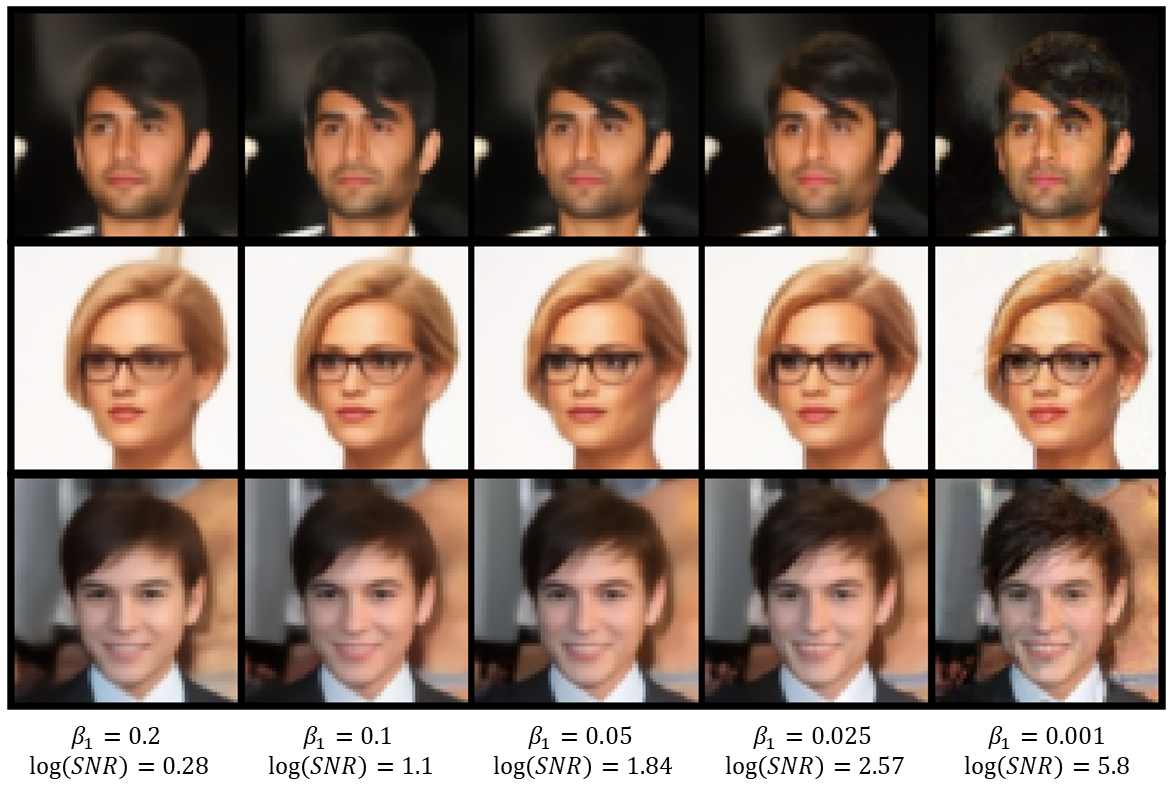
\includegraphics[width=0.8\linewidth]{pics/4_daed/experiments/daed_generations.png}
    \end{adjustbox}
    \caption{Examples of generations from \ours{} with the same noise value and different switching points.}
    \label{fig:daed_generations} 
% \vspace*{\baselineskip}
    \end{figure}
% \end{wrapfigure}

To get further insight into the qualitative performance, in Figure~\ref{fig:daed_generations} we demonstrate how the selection of the splitting point with respect to the Signal to Noise Ratio (SNR) affects the quality of final generations\footnote{Generations for all datasets are presented in Appendix~\ref{appx:generation}}. We present non-cherry-picked samples from \ours{} trained in the same manner as described in the previous paragraph. As expected, the more noise the DAE part (the denoiser) must deal with (see the values of $\beta_1$ in Figure~\ref{fig:daed_generations}), the fewer details in the generations there are. These samples again indicate that by replacing some steps with a denoiser, we get a trade-off between ''cleaning'' the corrupted image or, in fact, further generating details. It seems that there is a sweet spot for perceptually appealing images that contain details and are ''smooth'' at the same time, see $\beta_1=0.025$ in Figure~\ref{fig:daed_generations}. However, as it is typically difficult to provide convincing arguments by \textit{staring} at samples, we further propose to analyze quantitative measures.

\begin{table*}[t!]
  \centering
  \captionsetup{width=1.4\textwidth, margin={0pt, -.4\textwidth}}
  \caption{FID Precision (Prec) and Recall (Rec) scores. For each row, we indicate the length of the diffusion process (T) and the training objective (Loss). \textbf{Best results in bold}.}
  \label{tab:results_fmnist_cifar_celeba}
  \vskip -5pt
  \resizebox{1.4\textwidth}{!}{
  \begin{tabular}{l|c||c|ccc||c|ccc||c|ccc}
    \toprule
     \multicolumn{2}{c||}{Model} & \multicolumn{4}{c||}{Fashion Mnist} & \multicolumn{4}{c||}{CIFAR10} &   \multicolumn{4}{c}{CelebA} \\
    \midrule
    & Loss & T & FID $\downarrow$&Prec $\uparrow$ & Rec $\uparrow$ & T & FID $\downarrow$ & Prec $\uparrow$ & Rec $\uparrow$ & T & FID $\downarrow$ & Prec $\uparrow$ & Rec $\uparrow$\\

    \midrule
    DDGM & VLB & 500 & 8.9 & 68 & 53 & 1000 & 26 & 53 & 54 & 1000 & 23 & 51 &21\\
    \ours{} $\beta_1=0.1$ & VLB & 468 & 9.1 & \textbf{71} & 60 & 900 & 20 & 59 & 46 & 900 & 18 & 63 & \textbf{30}\\
    \ours{} $\beta_1=0.001$ & VLB & 499 & \textbf{7.5} & \textbf{71} & \textbf{64} & 999 & \textbf{15} & \textbf{60} & \textbf{60} & 999 & \textbf{16} & \textbf{70} & 27 \\
    \midrule
    DDGM & Simple & 500 & 7.8 & 72 & \textbf{65} & 1000 & \textbf{7.2} & \textbf{65} & \textbf{61} & 1000 & \textbf{4.9} & 66 & \textbf{57}\\
    \ours{} $\beta_1=0.1$& Simple & 468 & 9.6 & \textbf{73} & 58 & 900 & 19 & 62 & 50 & 900 & 22 & \textbf{67} & 27 \\
    \ours{} $\beta_1=0.001$ &Simple & 499 & \textbf{5.7} & 69 & 64 & 999 & 14.8 & \textbf{65} & 53 & 999 & 7.4 & \textbf{67} & 54 \\
    \bottomrule
  \end{tabular}}
% \vspace*{\baselineskip}
\end{table*}

In Table \ref{tab:results_fmnist_cifar_celeba}, we compare the performance of \ours{} against the DDGM on FashionMNIST, CIFAR10, and CelebA in terms of FID, Precision and Recall scores. We want to highlight that our goal is not to achieve SOTA results on the before-mentioned datasets but to verify whether we can gain some further understanding and, potentially, some improvement by splitting the denoising and generative parts. We consider two scenarios, namely, learning a DDGM and \ours{}s using either the variational lower bound (VBL) or the simplified objective (Simple) with various lengths of the diffusion. Interestingly, \ours{} outperforms the DDGM when these models are trained using the VBL loss. For the simplified objective, \ours{} trained with the same number of diffusion steps yields slightly lower performance than standard DDGMs. As indicated by the Precision/Recall, generations from \ours{} are as precise as those from DDGM. However, they lack certain diversity, probably due to the smoothing effect of the DAE part. Detailed results for other setups are presented in Appendix~\ref{appendix:extra_results}.\footnote{In Appendix~\ref{appx:large_models} we show that increasing the number of parameters of DDGMs to be comparable to \ours{} does not lead to significant performance improvements.}

\subsection{Does the noise removal in DDGMs generalize to other data distributions?}
The last question we are interested in is the generalizability of DDGMs to other data distributions. We refer to this concept as \textit{transferability} for short. In other words, the goal of this experiment is to determine whether we can reuse a model or its part on new data with as good performance as possible. In this experiment, we rely on the results presented in Section~\ref{sect:reasonable_to_use_denoiser} where roughly the first $10\%$ of steps could be seen as the denoising part. To further strengthen this perspective, we also utilize \ours{} with an explicit division into the denoising and generating parts.

\begin{table}[t]
  \centering
  \caption{Reconstruction errors measured by MAE~($\downarrow$), MS-SSIM~($\uparrow$) for images noised with $\beta_1=0.1$. \\
  	*To evaluate models trained on CIFAR10, we downscale CelebA to $32\times32$. \textbf{Best results in bold.}}
  \vskip -5pt
  \resizebox{\textwidth}{!}{
  \begin{tabular}{c|l||cccccc}
    \toprule
    & Target dataset & \multicolumn{2}{c}{CIFAR10} & \multicolumn{2}{c}{CIFAR100} & \multicolumn{2}{c}{CelebA*}\\
    \midrule
    Source Dataset& Model& MAE & MS-SSIM & MAE & MS-SSIM & MAE & MS-SSIM \\ 
    \midrule
    \multirow{3}{*}{CIFAR10} & DDGM VLB & 0.091 &0.94 & 0.097 &0.94 & 0.093 &0.95 \\
    & DDGM Simple & 0.085 & 0.95 & 0.097 & 0.94 & 0.096 & 0.95\\
    & \ours{} & \textbf{0.065} & \textbf{0.97} & \textbf{0.074} & \textbf{0.97} & \textbf{0.068} & \textbf{0.97}\\
    \midrule
    \multirow{3}{*}{ImageNet} & DDGM VLB & 0.113 & 0.93 & 0.110 & 0.93 & 0.077 & 0.96\\
    & DDGM Simple & 0.113 & 0.94 & 0.111 & 0.93 & 0.068 & 0.96\\
    & \ours{} & \textbf{0.071} & \textbf{0.97} & \textbf{0.071} & \textbf{0.97} & \textbf{0.050} & \textbf{0.98}\\
    \bottomrule
  \end{tabular}
  }
  \label{tab:transferability}
\end{table}

First, we consider the case in which we compare the reconstruction errors measured by the MAE and the MS-SSIM. In this scenario, we train a DDGM on a source dataset and then assess it on a target dataset. We use CIFAR10 or ImageNet (32x32 or 64x64) as source data and CIFAR10, CIFAR100, or CelebA as target data. For each image from the target dataset, we apply the DAE part of \ours{} to obtain the reconstruction or 793 steps of the forward and backward diffusion in the case of the DDGM, which corresponds to the same level of added noise. For this experiment, we use the pre-trained DDGM from \citet{nichol2021improved} that consists of 4000 steps and uses the cosine noise scheduler. The results are outlined in Table~\ref{tab:transferability}. First of all, there is no significant difference in the performance of DDGMs trained with either the VBL objective or the simplified objective. They achieve a quite satisfactory MAE and MS-SSIM scores. However, \ours{} outperforms the DDGMs, obtaining much better transferability. We explain it by the fact that probably, with each step in the denoising part DDGM adds details that are typical for source data while \ours{} focuses on removing noise and produces a smoother output. This outcome may further suggest that splitting DDGMs into two parts with two separate parameterizations is reasonable and even beneficial.

To get further insight into the transferability behavior, we present a few (non-cherry-picked) examples from CelebA in Figure~\ref{fig:transferability}a and four toy examples in Figure~\ref{fig:transferability}b. We use the same setup as explained in the previous paragraph (i.e., the pre-trained DDGM provided in \citet{nichol2021improved}), and the images are noised with $\beta_1=0.1$. In columns 3--6 in Figure~\ref{fig:transferability}a, we present reconstructions for the DDGM trained on CelebA, the DDGM trained on ImageNet, \ours{} trained on CelebA, and \ours{} trained on ImageNet, respectively. It becomes apparent that the DDGM trained on CelebA denoises the image by generating new details while \ours{} denoises by smoothing. 
Interestingly, \ours{} performs better than the DDGM when we use ImageNet-trained models to denoise CelebA.
In~Figure~\ref{fig:transferability}b, we depict several toy examples that were denoised with the DDGM and DAED trained on CIFAR10. We see that the DDGM adds many details that are artifacts from the source data. It seems that \ours{} does not suffer from that behavior.

\begin{figure}[t]
	\centering
	\begin{tabular}{cc}
	   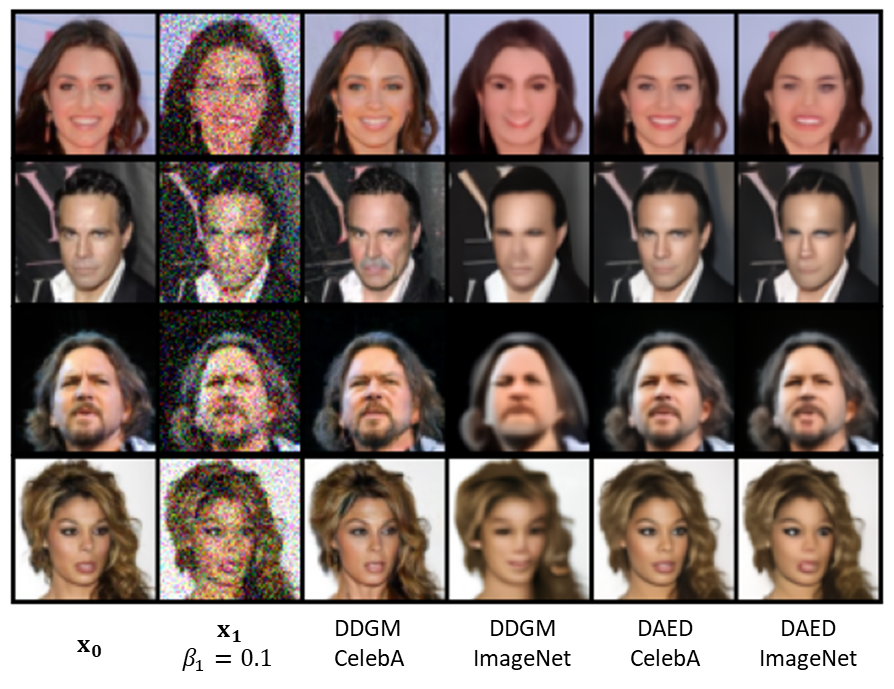
\includegraphics[width=0.56\linewidth, valign=c]{pics/4_daed/experiments/portability.png} & 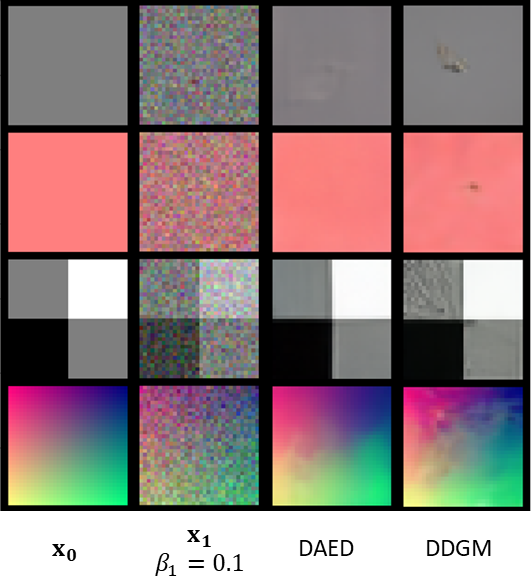
\includegraphics[width=0.38\linewidth, valign=c]{pics/4_daed/experiments/toy_example.png} \\
	    (a) Reconstructions on CelebA & (b) Toy examples
	\end{tabular}
	\caption{(a) Denoising of image with $0.1$ noise using either \ours{} or the corresponding number of the DDGM steps. (b) Four noisy toy examples denoised by \ours{} and the DDGM.}
	\label{fig:transferability}
\end{figure}
